\documentclass[]{elsarticle} %review=doublespace preprint=single 5p=2 column
%%% Begin My package additions %%%%%%%%%%%%%%%%%%%
\usepackage[hyphens]{url}

  \journal{Transport Findings} % Sets Journal name


\usepackage{lineno} % add
\providecommand{\tightlist}{%
  \setlength{\itemsep}{0pt}\setlength{\parskip}{0pt}}

\usepackage{graphicx}
\usepackage{booktabs} % book-quality tables
%%%%%%%%%%%%%%%% end my additions to header

\usepackage[T1]{fontenc}
\usepackage{lmodern}
\usepackage{amssymb,amsmath}
\usepackage{ifxetex,ifluatex}
\usepackage{fixltx2e} % provides \textsubscript
% use upquote if available, for straight quotes in verbatim environments
\IfFileExists{upquote.sty}{\usepackage{upquote}}{}
\ifnum 0\ifxetex 1\fi\ifluatex 1\fi=0 % if pdftex
  \usepackage[utf8]{inputenc}
\else % if luatex or xelatex
  \usepackage{fontspec}
  \ifxetex
    \usepackage{xltxtra,xunicode}
  \fi
  \defaultfontfeatures{Mapping=tex-text,Scale=MatchLowercase}
  \newcommand{\euro}{€}
\fi
% use microtype if available
\IfFileExists{microtype.sty}{\usepackage{microtype}}{}
\bibliographystyle{elsarticle-harv}
\ifxetex
  \usepackage[setpagesize=false, % page size defined by xetex
              unicode=false, % unicode breaks when used with xetex
              xetex]{hyperref}
\else
  \usepackage[unicode=true]{hyperref}
\fi
\hypersetup{breaklinks=true,
            bookmarks=true,
            pdfauthor={},
            pdftitle={An examination of the accessibility implications of a pilot COVID-19 vaccination program in Hamilton, Ontario},
            colorlinks=false,
            urlcolor=blue,
            linkcolor=magenta,
            pdfborder={0 0 0}}
\urlstyle{same}  % don't use monospace font for urls

\setcounter{secnumdepth}{0}
% Pandoc toggle for numbering sections (defaults to be off)
\setcounter{secnumdepth}{0}

% Pandoc citation processing
\newlength{\csllabelwidth}
\setlength{\csllabelwidth}{3em}
\newlength{\cslhangindent}
\setlength{\cslhangindent}{1.5em}
% for Pandoc 2.8 to 2.10.1
\newenvironment{cslreferences}%
  {}%
  {\par}
% For Pandoc 2.11+
\newenvironment{CSLReferences}[3] % #1 hanging-ident, #2 entry spacing
 {% don't indent paragraphs
  \setlength{\parindent}{0pt}
  % turn on hanging indent if param 1 is 1
  \ifodd #1 \everypar{\setlength{\hangindent}{\cslhangindent}}\ignorespaces\fi
  % set entry spacing
  \ifnum #2 > 0
  \setlength{\parskip}{#2\baselineskip}
  \fi
 }%
 {}
\usepackage{calc} % for calculating minipage widths
\newcommand{\CSLBlock}[1]{#1\hfill\break}
\newcommand{\CSLLeftMargin}[1]{\parbox[t]{\csllabelwidth}{#1}}
\newcommand{\CSLRightInline}[1]{\parbox[t]{\linewidth - \csllabelwidth}{#1}}
\newcommand{\CSLIndent}[1]{\hspace{\cslhangindent}#1}

% Pandoc header
\usepackage{float} \usepackage{xcolor} \floatplacement{figure}{H} \usepackage[margin=1.25in]{geometry}
\usepackage{booktabs}
\usepackage{longtable}
\usepackage{array}
\usepackage{multirow}
\usepackage{wrapfig}
\usepackage{float}
\usepackage{colortbl}
\usepackage{pdflscape}
\usepackage{tabu}
\usepackage{threeparttable}
\usepackage{threeparttablex}
\usepackage[normalem]{ulem}
\usepackage{makecell}
\usepackage{xcolor}



\begin{document}
\begin{frontmatter}

  \title{An examination of the accessibility implications of a pilot
COVID-19 vaccination program in Hamilton, Ontario}
    \author[McMaster University]{Antonio Paez\corref{1}}
   \ead{paezha@mcmaster.ca} 
    \author[University of Toronto Scarborough]{Christopher D. Higgins}
   \ead{cd.higgins@utoronto.ca} 
      \address[McMaster University]{School of Earth, Environment and
Society, McMaster University, Hamilton, ON, L8S 4K1, Canada}
    \address[University of Toronto Scarborough]{Department of Geography
\& Planning, University of Toronto Scarborough, 1265 Military Trail,
Toronto, ON M1C1A4}
      \cortext[1]{Corresponding Author}
  
  \begin{abstract}
  The Government of Ontario in Canada announced the pilot for a new
  vaccination program, with designated pharmacies across the province
  now able to offer COVID-19 vaccines. The accessibility of this program
  raises questions about travel times to vaccination sites and the
  distribution of these times among the population. In our examination
  of the City of Hamilton we find that selected sites do not serve rural
  and urban residents well; particularly, the associated cost of travel
  (in terms of travel time) is expected to be disproportionally borne by
  lower income urban populations and rural residents. Modest additions
  to the list of pilot sites in the city can substantially alleviate
  this inequity.
  \end{abstract}
  
 \end{frontmatter}

\hypertarget{questions}{%
\section{Questions}\label{questions}}

Along with the provision of health care facilities to treat severe cases
of COVID-19 (e.g., Ghorbanzadeh et al., 2021; Pereira et al., 2021a),
another front in the fight against the pandemic is the rolling out of
vaccination programs. The Government of Ontario, in Canada, implemented
in 2021 a pilot program to offer vaccines in pharmacies for people 60
years and older. In the first incarnation of this program, the province
approved 325 pharmacies in Toronto, Windsor-Essex, and Kingston (the
latter including the region of Frontenac-Lennox and Addington). The City
of Hamilton, the third most populous urban center in the province,
operated dedicated vaccination centers for people aged 70+ and mobile
pop-up clinics for people aged 75+; however, it did not have any
approved pharmacies under the pilot for other populations until April
1st 2021, with the announcement of 20 pharmacies in the city
\footnote{\url{https://www.cbc.ca/news/canada/hamilton/astrazeneca-vaccine-hamilton-1.5972704}}.
At the same time that the expansion of the pilot was announced, the
province extended eligibility for this program to people 55 years and
older.

Critics were swift to point out that the list of pharmacies approved for
Hamilton by the province were mostly located in lower density parts of
the city that are not well serviced by transit and are difficult to
reach by
foot\footnote{See inter alia: \url{https://twitter.com/RyanMcGreal/status/1378027149790224386?s=20} and \url{https://twitter.com/NrinderWard3/status/1378679195514060801?s=20}.}.
Indeed, as seen in Figure \ref{fig:pharmacies-and-regions}, a vast
majority of the pharmacies are in suburban Hamilton. Whether this is an
issue is less clear-cut when we consider that Hamilton's older
population skews suburban (see Figure \ref{fig:population-map}). Given
the target demographic for the program, it is possible that suburban
sites could be convenient for mature adults and the young old: the
population aged 55 to 69 in Hamilton is approximately 58,710 suburban,
35,490 urban, and only 8,360 rural. Nevertheless, the selection of sites
by the province raised some important
questions\footnote{The decision-making process to select these sites appears to have been opaque, and the Mayor of the city was caught flat footed by the announcement; see: \url{https://twitter.com/FredEisenberger/status/1378350123114242053?s=20}}.
As Yu et al. (2021) note, good geographical coverage is a key element
for a successful vaccination campaign; at the same time, siting
vaccinations sites in car-oriented locations may lead to inequities in
access by requiring people who do not own cars or who typically travel
by other modes (mostly lower income urban residents) to spend more of
their time reaching an approved pharmacy.

In this research, we investigate the accessibility implications of the
sites selected for the pilot vaccination program. Concretely, we ask:

\begin{itemize}
\tightlist
\item
  What is the estimated travel time needed to reach the nearest approved
  pharmacy, assuming that every person requires a vaccine?
\item
  What is the distribution of travel times across the population of the
  city?
\item
  How does the cost of time needed for travel and its distribution
  change with the addition of candidate vaccination sites in urban
  Hamilton?
\end{itemize}

We concentrate on the 55 to 69 years old population segment because the
older 70+ group have access to other dedicated facilities besides those
in the provincial pilot (including pop-up clinics for people 75+).

\begin{figure}

{\centering 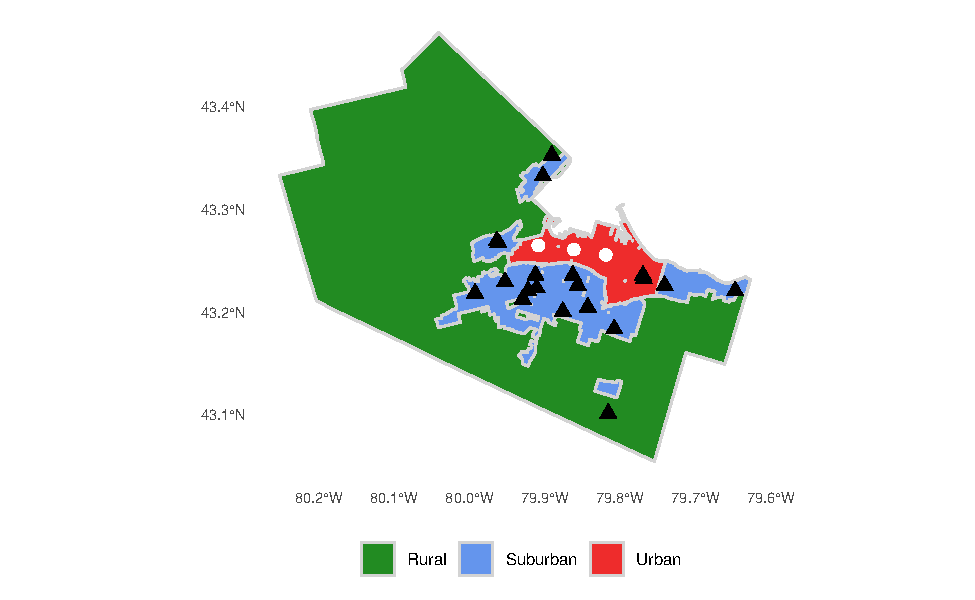
\includegraphics{Accessibility-Vaccination-Sites-Hamilton_files/figure-latex/pharmacies-map-1} 

}

\caption{\label{fig:pharmacies-and-regions}Regions with the City of Hamilton; the location of pharmacies in pilot is shown (black triangles) along with urban locations for scenario analysis (white circles).}\label{fig:pharmacies-map}
\end{figure}

\begin{figure}

{\centering 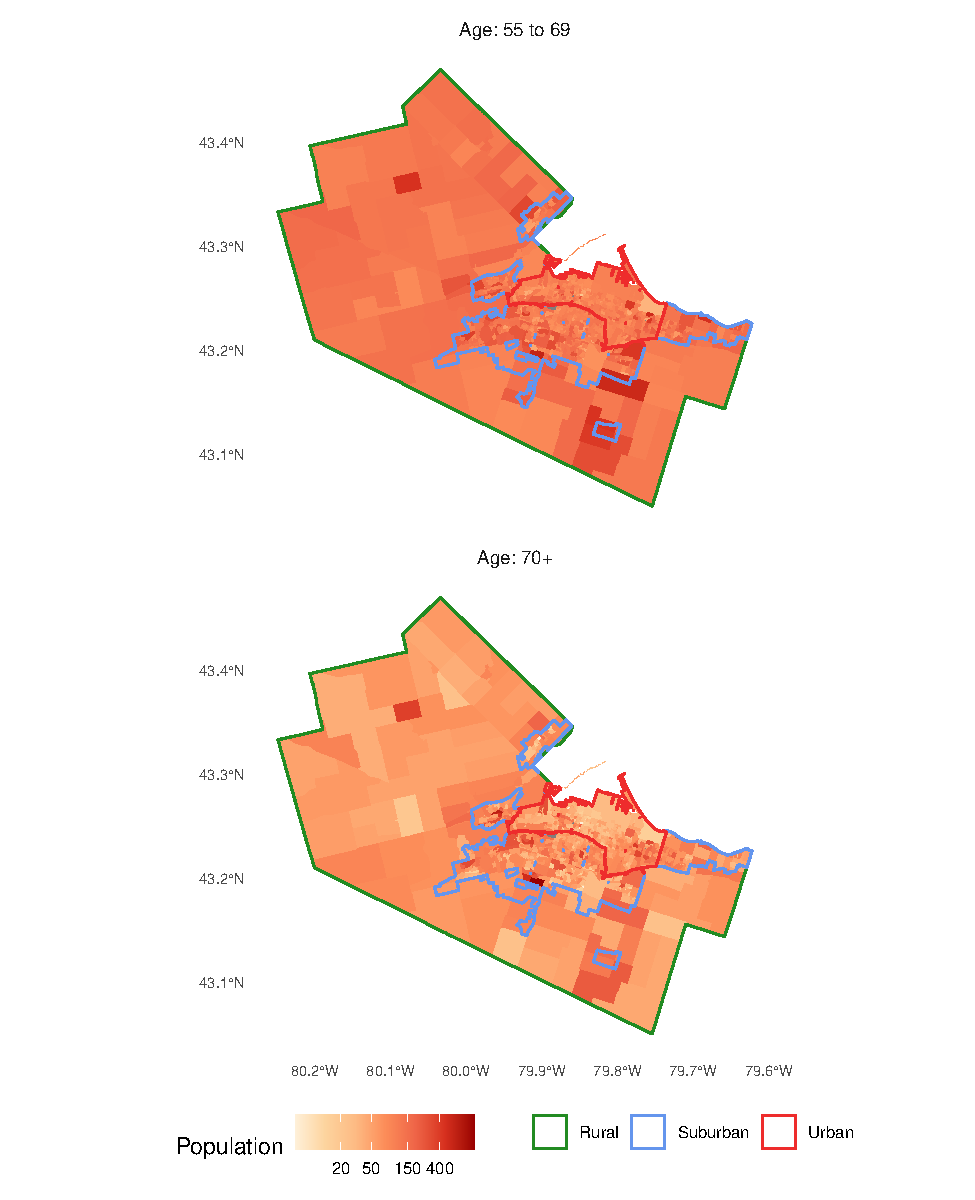
\includegraphics{Accessibility-Vaccination-Sites-Hamilton_files/figure-latex/population-map-1} 

}

\caption{\label{fig:population-map}Distribution of population aged 55+ in the City of Hamilton.}\label{fig:population-map}
\end{figure}

\hypertarget{methods}{%
\section{Methods}\label{methods}}

We use data from the following sources.

\begin{itemize}
\tightlist
\item
  Urban, suburban, and rural boundary definitions from the City of
  Hamilton\footnote{\url{https://open.hamilton.ca/}}
\item
  Population and median total household income for 2016 by Dissemination
  Area (DA) boundary using the \texttt{cancensus} package (von Bergmann
  et al., 2021)
\item
  Modal split by age for traffic analysis zones (TAZ) from the 2016
  Transportation Tomorrow Survey
  (TTS)\footnote{\url{http://dmg.utoronto.ca/}}
\item
  Locations of pilot pharmacies from public records
\item
  Locations of three additional major chain pharmacies for scenario
  testing
\item
  Residential units by land parcel
\end{itemize}

Using the population aged 55 to 69 y.o. we first calculate the average
number of people per dwelling and assign them proportionally to the
dwellings by parcel. Second, median household incomes and modal splits
across walking, transit, and car are joined to the parcels. Our data are
from 2016 (the most recent available), but we assume they are largely
representative of spatial, mobility, and demographic trends in the city.
In the absence of travel behavior information during the pandemic we
suggest this is an inevitable limitation of the analysis. Third, we use
the \texttt{r5r} (Pereira et al., 2021b) package to calculate the travel
time from each parcel to all pharmacies by three modes using a cutoff
value of 180 min and a maximum walking distance of 10,000 m. These
thresholds are chosen to maximize the coverage of the travel time
tables, but the analysis, as explained next, is based on travel to the
nearest approved pharmacy. Once we obtained travel time tables with
population, proportion of trips by mode, and income information, we
calculated the expected travel time \(ett\) from each parcel \(i\) to a
pharmacy \(j\) as follows: \[
ett_i = p^c_i \min(tt^c_{ij}) + p^t_i \min(tt^t_{ij}) + p^w_i \min(tt^w_{ij})
\] \noindent where \(p^k_i\) is the proportion of trips by mode \(k\) in
the TAZ of parcel \(i\), and \(tt^k_{ij}\) is the vector of travel times
from parcel \(i\) to the pharmacies. The expected travel time is thus
the weighted sum of travel times to the \emph{nearest} pharmacy, with
the weights given by the expected modal split in the TAZ.

The expected travel time \(i\) was multiplied by the assigned population
in parcel \(i\) to obtain a measure of person-hours of travel (\(PHT\))
that gives a cumulative cost (in travel time) for a population group.
This is as follows: \[
PHT_i = P_i\cdot ett_i
\]

Please note that this paper is a reproducible research document (see
Brunsdon and Comber, 2020) conducted using open source tools for
transportation analysis (Lovelace, 2021). The code and data necessary to
reproduce the analysis are available in a public
repository\footnote{\url{https://github.com/paezha/Accessibility-Pharmacies-Hamilton-Vaccines}}.

\hypertarget{findings}{%
\section{Findings}\label{findings}}

The top panel of Figure \ref{fig:maps-baseline} shows the average
multi-modal travel times (weighted by modal shares) by TAZ in Hamilton.
It is apparent that travel times tend to be lower in much of suburban
Hamilton and higher in the urban core and some rural parts of the city,
particularly to the west. This is unsurprising, given the higher
probability of travel by car and the predominantly suburban character of
the vaccination sites. However, even accounting for the distribution of
population, this leads to large disparities in the number of
person-hours of travel across the city, with a concentration of the
burden of travel in the urban core and the rural west (see bottom panel
of Figure \ref{fig:maps-baseline}).

The disparities are not trivial.

As seen in Table \ref{tab:distribution-results}, under the pilot program
approximately 36.42\% of people live in DAs in the bottom 40\% of the
median household income scale, but they account for 51.98\% of the total
person-hours of travel. In contrast, 44.5\% of people aged 55 to 69 in
DAs in the top 40\% of the median household income scale accrue only
35.03\% of the total person-hours of travel. Where the mean travel time
of residents of DAs with high median household income is 347 minutes,
residents of lower income DAs average 746 minutes in travel time. In
addition to longer average travel time, residents in lower income DAs
also see substantially larger variations in travel times, and some may
face considerably longer travel times (see top-left panel in Figure
\ref{fig:results}).

There are also important disparities by region. As shown in Table
\ref{tab:distribution-results}, the urban and rural populations in
Hamilton are approximately 42.75\% of the population but they bear
69.25\% of the total person-hours of travel, with also much greater
variability in expected travel times (Figure \ref{fig:results},
bottom-left panel).

For comparison purposes we consider a scenario with some modest
additions to the list of pharmacies in the provincial pilot. For the
scenario we choose three plausible sites (i.e., pharmacies that belong
to chains already used by the province for this program). We do not
conduct a systematic search of candidate locations. We note that some
papers propound the design optimal accessibility landscapes (e.g.,
Horner, 2008; Páez et al., 2013), but such an endeavor is beyond the
scope of a short findings paper. Instead, we repeat the analysis after
including the three urban sites shown in white circles in Figure
\ref{fig:pharmacies-and-regions}.

The results of this scenario appear in the last two columns of Table
\ref{tab:distribution-results} and the two right panels of Figure
\ref{fig:results}. While all income groups benefit from the addition of
these three sites with shorter mean trip durations, the most remarkable
difference is the large reduction in the disparities between residents
in DAs with lower levels of income. The top-right panel of Figure
\ref{fig:results} shows that the distribution of expected travel time is
now more in line for all income groups, even if the bottom two income
quintiles still have somewhat wider spreads. Unsurprisingly, the
addition of three urban vaccination sites does not have a large impact
for rural residents. The scenario also suggests that important
reductions in the need for travel can be achieved. While this is true
for all three modes of transportation (see Table
\ref{tab:distribution-results-by-mode}), the reductions are more
substantial for travel by transit and walking. At a time that
non-pharmaceutical interventions call for reductions in mobility, it is
clearly in the public interest to reduce the need to travel even for
this essential purpose.

The results indicate that the locations chosen by the province for the
pilot vaccination program do not serve urban or rural residents of the
city well, and there are some important questions regarding equity of
access to the program. As shown, a disproportionate burden in the cost
of travel (in terms of travel time) fall on lower income urban
populations and rural populations. Selection of three sensible urban
locations does much to alleviate disparities in the burden of
transportation - and the fact that this is so despite the lack of a
systematic search for optimal locations does not speak well of the
effort put by the province in the choice of vaccination sites. The
situation is different for rural populations, mainly because there are
not many candidate locations in rural parts of the city; in this case,
it is likely that increasing access for residents there will necessitate
an expansion of the existing mobile vaccination pop-up clinic
program\footnote{\url{https://www.hamilton.ca/government-information/news-centre/news-releases/hamiltons-covid-19-vaccination-program-expansion-1}}.

\begin{figure}

{\centering 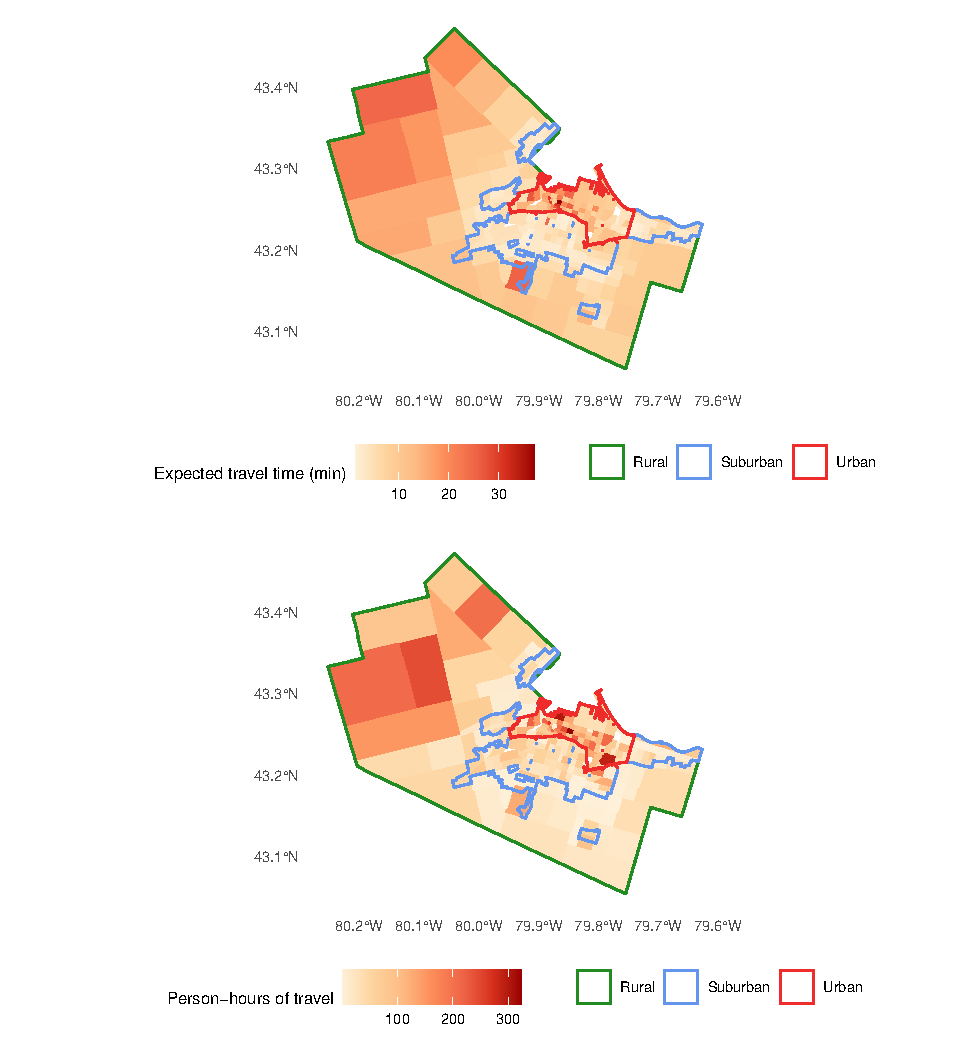
\includegraphics{Accessibility-Vaccination-Sites-Hamilton_files/figure-latex/figure-maps-baseline-1} 

}

\caption{\label{fig:maps-baseline}Average expected travel time by TAZ (in minutes) and total person-hours of travel by TAZ.}\label{fig:figure-maps-baseline}
\end{figure}

\begin{table}

\caption{\label{tab:table-results}\label{tab:distribution-results}Distribution of person-hours of travel (PHT) by median total household income and region: pilot locations only (baseline), and scenario with three urban locations added}
\centering
\resizebox{\linewidth}{!}{
\begin{tabular}[t]{lccccc}
\toprule
\multicolumn{2}{c}{ } & \multicolumn{2}{c}{Pilot Program} & \multicolumn{2}{c}{Scenario} \\
\cmidrule(l{3pt}r{3pt}){3-4} \cmidrule(l{3pt}r{3pt}){5-6}
Group & Population & Total PHT & Minutes per person & Total PHT & Minutes per person\\
\midrule
\addlinespace[0.3em]
\multicolumn{6}{l}{\textbf{Income Quintile}}\\
\hspace{1em}\cellcolor{gray!6}{Top 20\%} & \cellcolor{gray!6}{23297.315} & \cellcolor{gray!6}{2243.86} & \cellcolor{gray!6}{5.78} & \cellcolor{gray!6}{2146.56} & \cellcolor{gray!6}{5.53}\\
\hspace{1em}Second 20\% & 22356.413 & 2471.95 & 6.63 & 2351.86 & 6.31\\
\hspace{1em}\cellcolor{gray!6}{Third 20\%} & \cellcolor{gray!6}{19570.061} & \cellcolor{gray!6}{1749.50} & \cellcolor{gray!6}{5.36} & \cellcolor{gray!6}{1563.98} & \cellcolor{gray!6}{4.80}\\
\hspace{1em}Fourth 20\% & 17729.139 & 2928.96 & 9.91 & 1950.31 & 6.60\\
\hspace{1em}\cellcolor{gray!6}{Bottom 20\%} & \cellcolor{gray!6}{19629.952} & \cellcolor{gray!6}{4068.55} & \cellcolor{gray!6}{12.44} & \cellcolor{gray!6}{2388.42} & \cellcolor{gray!6}{7.30}\\
\addlinespace[0.3em]
\multicolumn{6}{l}{\textbf{Region}}\\
\hspace{1em}Rural & 8356.963 & 1730.27 & 12.42 & 1730.24 & 12.42\\
\hspace{1em}\cellcolor{gray!6}{Suburban} & \cellcolor{gray!6}{58711.629} & \cellcolor{gray!6}{4138.48} & \cellcolor{gray!6}{4.23} & \cellcolor{gray!6}{4138.39} & \cellcolor{gray!6}{4.23}\\
\hspace{1em}Urban & 35491.942 & 7588.59 & 12.83 & 4527.02 & 7.65\\
\bottomrule
\multicolumn{6}{l}{\rule{0pt}{1em}\textit{Note: }}\\
\multicolumn{6}{l}{\rule{0pt}{1em}The population totals differ due to small differences in the classification of the regions}\\
\end{tabular}}
\end{table}

\begin{table}

\caption{\label{tab:table-results-by-mode}\label{tab:distribution-results-by-mode}Distribution of person-hours of travel (PHT) by mode of transportation: pilot locations only (baseline) and scenario with three urban locations added}
\centering
\begin{tabular}[t]{lccc}
\toprule
Mode & Baseline PHT & Scenario PHT & Reduction in PHT\\
\midrule
\cellcolor{gray!6}{Car} & \cellcolor{gray!6}{8535.429} & \cellcolor{gray!6}{7092.220} & \cellcolor{gray!6}{-16.91\%}\\
Transit & 2730.205 & 2107.684 & -22.8\%\\
\cellcolor{gray!6}{Walking} & \cellcolor{gray!6}{2197.179} & \cellcolor{gray!6}{1201.223} & \cellcolor{gray!6}{-45.33\%}\\
\bottomrule
\end{tabular}
\end{table}

\begin{figure}

{\centering 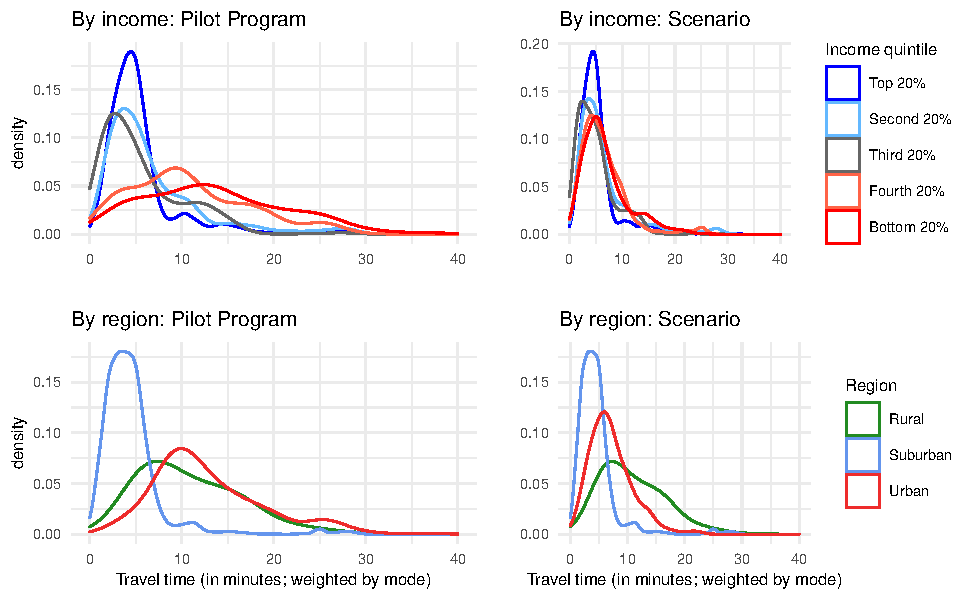
\includegraphics{Accessibility-Vaccination-Sites-Hamilton_files/figure-latex/figure-results-1} 

}

\caption{\label{fig:results}Distribution of expected travel time for different population groups.}\label{fig:figure-results}
\end{figure}

\hypertarget{references}{%
\section*{References}\label{references}}
\addcontentsline{toc}{section}{References}

\hypertarget{refs}{}
\begin{CSLReferences}{1}{0}
\leavevmode\hypertarget{ref-Brunsdon2020opening}{}%
Brunsdon, C., Comber, A., 2020. Opening practice: Supporting
reproducibility and critical spatial data science. Journal of
Geographical Systems 1--20.
doi:\href{https://doi.org/10.1007/s10109-020-00334-2}{10.1007/s10109-020-00334-2}

\leavevmode\hypertarget{ref-Ghorbanzadeh2021spatial}{}%
Ghorbanzadeh, M., Kim, K., Erman Ozguven, E., Horner, M.W., 2021.
Spatial accessibility assessment of COVID-19 patients to healthcare
facilities: A case study of florida. Travel Behaviour and Society 24,
95--101. doi:\url{https://doi.org/10.1016/j.tbs.2021.03.004}

\leavevmode\hypertarget{ref-Horner2008optimal}{}%
Horner, M.W., 2008. 'Optimal' accessibility landscapes? Development of a
new methodology for simulating and assessing jobs-housing relationships
in urban regions. Urban Studies 45, 1583--1602.
doi:\href{https://doi.org/10.1177/0042098008091492}{10.1177/0042098008091492}

\leavevmode\hypertarget{ref-Lovelace2021open}{}%
Lovelace, R., 2021. Open source tools for geographic analysis in
transport planning. Journal of Geographical Systems.
doi:\href{https://doi.org/10.1007/s10109-020-00342-2}{10.1007/s10109-020-00342-2}

\leavevmode\hypertarget{ref-Paez2013exploring}{}%
Páez, A., Esita, J., Newbold, K.B., Heddle, N.M., Blake, J.T., 2013.
Exploring resource allocation and alternate clinic accessibility
landscapes for improved blood donor turnout. Applied Geography 45,
89--97. doi:\url{http://dx.doi.org/10.1016/j.apgeog.2013.08.008}

\leavevmode\hypertarget{ref-Pereira2021geographic}{}%
Pereira, R.H.M., Braga, C.K.V.S., Mendes and Serra, L., Amaral, P.B.,
Gouveia, N., Paez, A., 2021a. Geographic access to COVID-19 healthcare
in brazil using a balanced float catchment area approach. Social Science
\& Medicine 273, 113773.
doi:\url{https://doi.org/10.1016/j.socscimed.2021.113773}

\leavevmode\hypertarget{ref-Pereira2021r5r}{}%
Pereira, R.H.M., Saraiva, M., Herszenhut, D., Braga, C.K.V., Conway,
M.W., 2021b. r5r: Rapid realistic routing on multimodal transport
networks with r\textsuperscript{5} in r. Findings.
doi:\href{https://doi.org/10.32866/001c.21262}{10.32866/001c.21262}

\leavevmode\hypertarget{ref-vonBergmann2021cancensus}{}%
von Bergmann, J., Shkolnik, D., Jacobs, A., 2021. Cancensus: R package
to access, retrieve, and work with canadian census data and geography.

\leavevmode\hypertarget{ref-Yu2021sustained}{}%
Yu, J.H., Jeong, H.J., Kim, S.J., Lee, J.Y., Choe, Y.J., Choi, E.H.,
Cho, E.H., 2021. Sustained vaccination coverage during the coronavirus
disease 2019 epidemic in the republic of korea. Vaccines 9, 8.
doi:\href{https://doi.org/10.3390/vaccines9010002}{10.3390/vaccines9010002}

\end{CSLReferences}


\end{document}

